%%% DOCUMENT BEGIN

\documentclass{article}

\usepackage[utf8]{inputenc}

\usepackage{geometry}
\geometry{a4paper}

\usepackage{graphicx}

%%% PACKAGES
\usepackage{booktabs} % for much better looking tables
\usepackage{array} % for better arrays (eg matrices) in maths
\usepackage{paralist} % very flexible & customisable lists (eg. enumerate/itemize, etc.)
\usepackage{verbatim} % adds environment for commenting out blocks of text & for better verbatim
\usepackage{subfig} % make it possible to include more than one captioned figure/table in a single float

%%% HEADERS & FOOTERS
\usepackage{fancyhdr} % This should be set AFTER setting up the page geometry
\pagestyle{fancy} % options: empty , plain , fancy
\renewcommand{\headrulewidth}{0pt} % customise the layout...
\lhead{}\chead{}\rhead{}
\lfoot{}\cfoot{\thepage}\rfoot{}

%%% SECTION TITLE APPEARANCE
\usepackage{sectsty}
\allsectionsfont{\sffamily\mdseries\upshape}

%%% ToC (table of contents) APPEARANCE
\usepackage[nottoc,notlof,notlot]{tocbibind} % Put the bibliography in the ToC
\usepackage[titles,subfigure]{tocloft} % Alter the style of the Table of Contents
\renewcommand{\cftsecfont}{\rmfamily\mdseries\upshape}
\renewcommand{\cftsecpagefont}{\rmfamily\mdseries\upshape} % No bold!


%%% END Article customizations


%%%%%%%%%%%%%%%%%%%%%%%%%
%%%          Fill in the title details                      %%%

\def \thetitle {INF-1400 Object oriented programming}
\def \thesubtitle {Assignment 3 - Mayhem clone}
\def \theauthor {Marius Mæland and Raymon S. Hansen}
\def \pagecount {3}

%%%%%%%%%%%%%%%%%%%%%%%%%

%\pagestyle{fancy}
\pagestyle{fancyplain} % options: empty , plain , fancy
\renewcommand{\headrulewidth}{1pt} % customise the layout...
\renewcommand{\footrulewidth}{0pt}
\lhead{\fancyplain{}{\thetitle{} -- \thesubtitle{}}}\chead{}\rhead{\fancyplain{}{\theauthor{}}}
\lfoot{}\cfoot{Page {\thepage} of \pagecount}\rfoot{}

\begin{document}

%%% TITLE PAGE

\begin{titlepage}
\begin{center}



\textsc{\\[3.5cm] \huge University of Tromsø}\\[1.5cm]

\textsc{\LARGE \thetitle}\\[0.5cm]

\textsc{\Large \thesubtitle}\\[1.5cm]

\LARGE{\theauthor} \\[0.5cm] \large{Department of Computer Science}



\vfill
{\large \today}

\end{center}
\thispagestyle{empty}
\end{titlepage}

\newpage{}


%%% TABLE OF CONTENTS

%\tableofcontents


\newpage{}

%%% DOCUMENT BODY

%%% Set counter to 1
\setcounter{page}{1}

\section{Introduction}

Short introduction to the assignment, motivation and expected results.\\

The assignment is to implement a clone of the old game Mayhem, but in this case we ended up with a space shooter death match type of game, however all of the requirements of the assignment are met. 

\subsection{Requirements}

Outline the detailed requirements specified in the assignment text. \\

Requrements for this assignment is to create a multiplayer game where each player can control their spaceship with four buttons, when thrusting the spaceships should move in the direction it is pointing, and are to be rotated right or left to control where to go. The ships should also be able to fire bullets.\\

Other requirements for the game:

\begin{itemize}

\item Two space ships
\item Four controls for each player
\item Controls: rotate left, rotate right, thrust and fire
\item Minimum one obstacle
\item Spaceship can crash with other objects on the screen
\item Gravity that acts on spaceships
\item A score for each player displayed on screen
\item Limited amount of fuel to the spaceships
\item Refuel station/ refuel pick up

\end{itemize}

There are also some requirements for the code:

\begin{itemize}

\item The code should be split in minimum two files
\item The main loop must have timing
\item The game shall be started using: 
\begin{verbatim} if__name__ == '__main__':\end{verbatim}
\item All visible objects shall subclass the pygame.sprite.Sprite class
\item All modules, classes and methods shall contain docstrings

\end{itemize}

\section{Technical Background}

Which topics are covered in this assignment. Should be short and cover the necessary topics without mentioning your specific implementation and design.\\

One of the requirements was that all moving objects in the game should sub-class
pygames sprite module. The pygame Sprite module is designed to make simple game 
design easier for developers. It includes built in functions for referring to 
and working with coordinates, displaying images for a better graphical look as
well as detecting collisions and working with objects/sprites in groups. 

Sprite groups is practical because it makes the use of polymorphism very easy.
The sprite module has a built in draw function which blits each sprites "image" 
attribute on a surface. We have also used this to simplify per frame update calls
on many different objects.

Allthough not a specific requirement, we have implemented and thoroughly enjoyed 
making animations with sprite sheets. Linking the actual code and the image 
files has given us valuable insight into how code interacts with "the outside world".
Cutting specific sections of a sprite sheet proved difficult at times, as each sheet
had a different layout, size, padding, alpha channels etc. 

\section{Design}

How did you solve the assignment? Describe the architecture and any design choices you've made. Show figures of the proposed architecture.\\ 

We chose to design the code so that each class had its own file to make the code easy to read, and then imported every file in to the game file to gather everything and run it in the game class. Each object that was needed got its own class, like player, explosion, bullet etc.. \\

\subsection{Player}
The player has all the attributes needed to make a spaceship, along with all of the methods needed to make it move, rotate, shoot, die and so on. To add the flame sprite to the space ship sprite and make it rotate, we had to create a new surface then blit the ship and the flame on the new surface and then rotate  the surface, this was partly done to avoid complex calculations regarding the placements of the sprites in relation to each other. The player makes an instance of bullets because the player is the one that knows where the bullets are to spawn on the screen and wich direction to send the bullets.

\subsection{Bullet}
The bullet have all the attributes and methods for the bullet behavior, and when bullet is called it loads and cuts the sprites in to a list to animate it.

\subsection{Asteroid}
Asteroid are animated, it takes in a list of the sprites to do the animation, but animates itself. The asteroid class takes inn width and height to make random scaled asteroids, and has a respawn method that respawns the asteroids at random location over or under the screen, with random x and y speed, but the y speed is set to posivite or negative in relation to witch side of the screen they spawn on, this is to make the asteroids always pass through the screen.

\subsection{Explosion}
The explosion class is just anitmating the explosion at the location it is called to, the explosion class also takes in width and height to scale it after the objects that explode.

\subsection{Animation}
This class animates pick up crystals, and the green gravity hole. It has the attributes for the crystals that apply the players random health and fuel on pick up, and have a static ammo amount. The crystals respawns on random location after picked up.

\subsection{config}
Config is the file with all the global variables, to prevent magic numbers, and makes it easy to just go into the config file to tweak the game. For more info on tweaking see README.

\subsection{Game}
The Game glass is the class that handles all of the things that happend in the game, it creats a screen, loads almost all of the sprites when start up, handles keypress, collision checks, where to create the explosions, sets up player information, creates instances of the objects and draws everything on the screen. 

\begin{figure}[h]
\begin{center}
\fbox{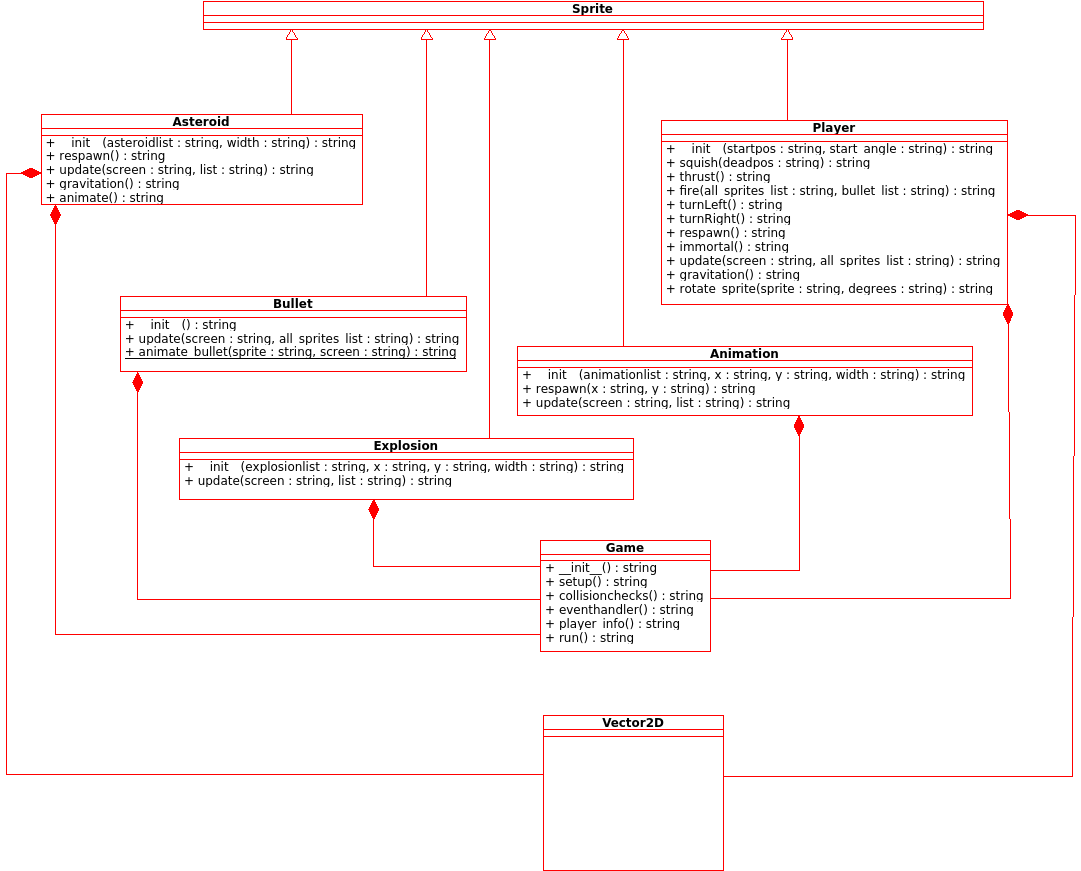
\includegraphics[width=177px]
{classdiagram.png}}
\end{center}
\caption{The class he}\label{fig:ackseq}
\end{figure}




\section{Implementation}

How did you implement, deploy and run your application? No need to refer to actual lines of code.\\ 

The assignment was written in python using Sublime Text build 3103 on Linux Mint 17 ”Qiana” and Linux Xubuntu 14.04 running kernel version 3.13.0-24 generic GNU/Linux. It also uses the pygame-library.

The various images and sprite sheets have all been edited using 
GIMP(GNU Image Manipulation Program). 

Profiling tools pydoc and cprofiler. 
%TODO: Add more!

\section{Discussion}

Any advantages or disadvantages with your design?\\

During tha writing of this assignment we have endeavoured to keep the architecture simple and easily understandable. In addition, we wanted it to be easy to expand with new ideas and elements. One of the reasons for working in a team was to experience how to manage one project with more writers. This forced us to carefully considder how encapsulation is handled. It must be possible for one person to work on some 
part of the code and the other works on another part, without worrying about making changes that ruin both writers contributions. As a result, the code has a fairly solid design on the whole. The game-class manages all the other classes as well as their interactions with each other(mainly when they crash!). \\

The explosion-class is a good example of solid and reusable code. It takes in alist of the frames to animate the explsion(this can then be any animation you like)as well as the point where you want it and the size. This made it very simple toanimate explsions when asteroids blow up, players die etc. The puff of dust when 
asteroids bump into eachother, is also an instance of the explosion-class.\\

A similar concept is used for the power ups as they are all instances of the animation-class They each get sent a different coloured list of frames to animate the crystals as well as placement and size. \\

A possible improvement on the explosion and animation would be to have a more general animation parent-class from which one could make power ups, explosions and so on inherit. Loading images and cutting subsurfaces from a sprite-sheet are heavy operations, therefore we have tried to do most of the loading in the game-class setup-method. The preloaded lists are then sent to each class where they are needed. The actual cutting of the animation-sheets are mostly done using nested for-loops to traverse
the image. We made some attempts at abstracting this process out as it is done several times. This proved difficult however because of great variasions in the layout of the sprite-sheets. As a result, the setup-method has it's own sheetcutter method, there's aslo a general img list and some for-loops. This is a bit messy and should have been abstracted out or the sprite-sheets could be changed to fit within a chosen standard. 


\section{Conclusion}

Sum up by restating the problem and solution. Follow up with a brief summary of the solution along with lessons learned.


%%% BIBLOGRAPHY

\newpage{}


\begin{thebibliography}{9}

\bibitem{coursebook}
 Robert Sedgewick 
  \emph{Algorithms in C - parts 1-4}.
  Addison-Wesley Publishing Company,
  3. Edition,
  1998.

\end{thebibliography}

\end{document}
